\documentclass[ %
    11pt,%
    a4paper,%
    BCOR=12mm,%
    DIV=12,%
    headsepline,%
    parskip=half,%    
    %draft=true,%
]{article}

\usepackage[utf8]{inputenc}
\usepackage[T1]{fontenc}
\usepackage{lmodern}
\usepackage{braket}
\usepackage{ulem}
%%englisches Protokoll
%\usepackage[british,UKenglish,USenglish,english,american]{babel}
% %
%%deutsches Protokoll
\usepackage[ngerman]{babel}
% %
\usepackage{amssymb,amsmath,setspace}
\usepackage{engrec}
\usepackage{enumerate}
\usepackage{empheq}
\usepackage{picins}
\usepackage{floatflt}
\usepackage{graphicx}
\usepackage{color}
\usepackage{natbib}
\usepackage{pdfpages}
\usepackage{hyperref}
\graphicspath{{Bilder/}}%% Allgemeine Bilder
\usepackage[paper=a4paper,left=25mm,right=25mm,top=25mm,bottom=25mm]{geometry}
% Seiten Layout
\usepackage[automark]{scrpage2} 


\begin{document}


\begin{titlepage}

\begin{center}




\includegraphics[width=0.3\textwidth]{Bilder/logo}\\[1.2cm]    

\textsc{\LARGE Albert-Ludwigs-Universit\"at Freiburg}\\[1.75cm]

\textsc{\Large Physikalisches Fortgeschrittenen-Praktikum I}\\[0.75cm]



\newcommand{\HRule}{\rule{\linewidth}{0.5mm}}
\HRule \\[0.5cm]
{ \huge \bfseries Szintillationszähler}\\[0.5cm]

\HRule \\[1.75cm]


\begin{minipage}{0.4\textwidth}
\begin{flushleft} \large
\emph{Studenten:}\\
Daniel \textsc{Uhl}\\ \setlength{\parindent}{1.25cm} \& 
\setlength{\parindent}{0cm} \\ Jan P\'eter \textsc{Szabados} 
\end{flushleft}
\end{minipage}
\hfill
\begin{minipage}{0.4\textwidth}
\begin{flushright} \large
\emph{Tutor:} \\
Matthias \textsc{Gorzellik}\\
\end{flushright}
\end{minipage}

\vfill


{\large \today}

\end{center}

\end{titlepage}

\pagenumbering{Roman}

%Seitenlayout
\pagestyle{scrheadings} 
\clearscrheadfoot 
\ihead{\headmark}

\tableofcontents
\newpage
\pagenumbering{arabic}
\section{Aufgabenstellung}
\begin{enumerate}
 \item Justage des SQUID per Control Panel am PC. Maximierung des SQUID-Patterns.
 \item Bestimmung des Dipolmoments/der Feldstärke der Leiterschleife mit den fünf Widerständen und Vergleich mit den berechneten Werten.
 \item Bestimmung der Dipolmomente/Feldstärken weiterer Proben.
 \item Darstellung der Stärke des Magnetfeldes in Abhängigkeit des Drehwinkels in Polardarstellung.
\end{enumerate}
\section{Theoretische Grundlagen}
\subsection{Supraleiter}
Man nennt Materialien, deren elektrischer Widerstand unterhalb einer materialabhängigen kritischen Temperatur $T_{C}$ unmessbar klein wird, Supraleiter. Dabei verhalten sie sich wie ideale Diamagneten: Wird ein äußeres Magnetfeld angelegt, wird ein Strom in dem Supraleiter induziert, sodass im Inneren des Leiters ein Magnetfeld induziert wird, welches das äußere Feld genau kompensiert. Bei der Verdrängung Magnetfeldes aus dem Inneren des Supraleiters spricht man vom 'Meissner-Ochsenfeld-Effekt'.\\
Das Prinzip der Supraleitung basiert auf sogenannten 'Cooper-Paaren', makroskopischen Zuständen von zwei Elektronen, welche über hunderte Nanometer hinweg miteinander verbunden sind. Die Entstehung und Wirkung der Cooper-Paare wird durch die sogenannte 'BCS-Theorie' beschrieben, welche noch ausführlich diskutiert wird.\\
Es kann durch steigende Temperatur (für $T>T_{C}$), aber auch durch große externe Ströme, ein starkes äußeres Magnetfeld oder ein externes elektromagnetisches Wechselfeld der Größenordnung $\omega\approx \Delta E/\hbar$, mit welchem Elektronen über die 'Bandlücke' des Supraleiters angeregt werden, die Supraleitung unterbrochen werden.\\
~\\
Es werden zwei Arten von Supraleitern unterschieden:\\
\textbf{Typ I}\\
Das innere Magnetfeld sinkt unterhalb einer kritischen äußeren Magnetfeldstärke $H_{C}$ auf 0 (wenn $T<T_{C}$). Das Magnetfeld dringt  nur wenige Nanometer in den Leiter ein.\\
~\\
\textbf{Typ II}\\
Diese Art von Supraleiter wird auch 'Hochtemperatursupraleiter' genannt, da die kritischen Temperaturen deutlich höher sind als diejenigen für Supraleiter von Typ I. \\
Es werden zwei Stufen für das innere Magnetfeld unterschieden:  Unterhalb der externen Feldstärke $H_{C_{2}}$ sinkt die innere Feldstärke auf kleine Werte, unterhalb von $H_{C_{1}}$ auf null. Zwischen diesen beiden Feldstärken kommt es zur Bildung von Flussfäden im Leiter, welche lokal für einen kleinen Feldbeitrag sorgen. 
\subsection{BCS-Theorie}
Wie bereits erwähnt, wird die Supraleitung mittels Cooper-Paare, welche aus zwei Elektronen bestehen, die über hunderte Nanometer miteinander wechselwirken, durch die BCS-Theorie (benannt nach ihren Entwicklern John \textbf{B}ardeen, Leon N. \textbf{C}ooper und John R. \textbf{S}chrieffer) erklärt.\\
Die gegenseitige Anziehung der Elektronen beruht auf der Trägheit der positiv geladenen Atomrümpfe. Kommt es zu Gitterschwingungen im Kristall, so wandern die Atomrümpfe langsamer in ihre Ausgangsposition zurück als die Elektronen. Aus diesem Grund ziehen - bildlich gesprochen - Elektronen einen Schweif positiver Polarität hinter sich her. Dieser kann ein Elektron ähnlicher Energie und entgegengesetztem Spin anziehen, wodurch sich ein Cooper-Paar bildet. \\
Um möglichst viele solche Paare zu erhalten, muss eine tiefe Temperatur vorherrschen, damit alle Zustände bis zur Fermi-Energie gefüllt sind. Auf diese Weise gibt es viele Elektronen ähnlicher Energie und kaum thermische Anregung: Die schwache Wechselwirkung zwischen den beiden Elektronen, welche das Cooper-Paar formen, wird also nicht aufgebrochen. Die einzelnen Elektronen bilden nun nicht mehr Fermionen, sondern dank der Spinkopplung miteinander ein Boson. Die Wechselwirkungsenergie ist dabei kleiner als die der einzelnen Ladungsträger.\\
Da die Bosonen nicht dem Pauli-Prinzip unterliegen, können beliebig viele Cooper-Paare denselben Zustand, auch den Grundzustand, einnehmen. Dadurch kommt es zu keiner Wechselwirkung mit dem Rest des Leiters mehr, was der Grund für den unmessbar kleinen elektrischen Widerstand ist. \\
Kommt es zum Zusammenbrechen der Supraleitung, werden eigentlich die Cooper-Paare aufgebrochen. Bei dem Entstehen eines Cooper-Paares wird Energie frei. Wird diese Energie einem Cooper-Paar zugeführt, kann dieses aufgebrochen werden. Unterschiedliche Methoden hierfür wurden im Unterkapitel 'Supraleiter' beschrieben.
\subsection{Flussquantisierung}
Der in diesem Versuch verwendete Supraleiter hat die Form eines Ringes. Der magnetische Fluss kann somit mithilfe des Stoke'schen Satzes über das geschlossene Integral des Vektorfelds $\vec{A}$ über die Leiterschleife berechnet werden: 
\[\oint\vec{A}d\vec{l}=\Phi_{B}.\]
Da sich, wie bereits diskutiert, alle Cooper-Paare im gleichen Zustand befinden, können sie als Gesamtwelle betrachtet werden. Somit ist es klar, dass sich die Phase $\theta$ bei einem Umlauf nur um Vielfache von $2\pi$ ändern kann: 
\[\oint\triangledown\theta d\vec{l}=\Delta\theta=n\cdot 2\pi,\] 
wobei $n\in\mathbb{N}$.\\
Somit ergibt sich die Quantisierung des magnetischen Flusses im geschlossenen Supraleiter in sogenannten Flussquanten: 
\[\left|\Phi_{B}\right|=n\frac{\hbar}{2e}=n\Phi_{0},\]
wobei $\Phi_{0}=2,067833667\cdot10^{-15}Tm^{2}$ (Quelle: [ver]).
\subsection{Josephson-Effekt}
Der Josephson-Effekt tritt auf, wenn ein dünner Isolator ('Josephson-Kontakt') zwischen zwei Supraleiter gebracht wird.
\begin{figure}[h]
\begin{center}
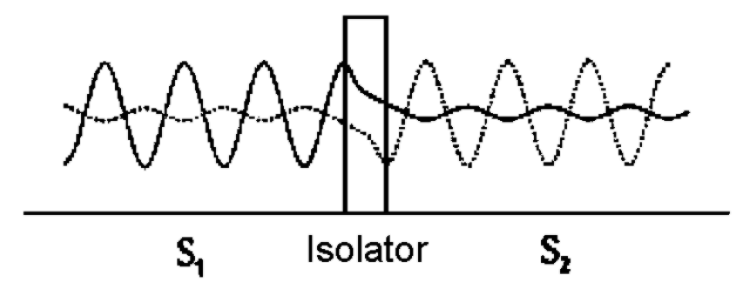
\includegraphics[scale=0.6]{Bilder/josephson}
\caption{Josephson-Kontakt zwischen zwei Supraleitern. Quelle: [ver].}
\end{center}
\end{figure}
~\\
Aufgrund der geringen Breite des Kontakts (wenige Nanometer) können Cooper-Paare mit hoher Wahrscheinlichkeit durch ihn tunneln, wodurch ein Tunnelstrom verursacht wird.\\
Wenn der Josephson-Kontakt, wie in diesem Experiment, zwischen zwei identischen Supraleitern ohne Potentialdifferenz liegt (dies ist hier der Fall wegen der Ringform des Supraleiters), so hängt der Tunnelstrom ausschließlich von der Phasendifferenz der einlaufenden Wellen ab. Der Josephson-Kontakt verhält sich zwar für den Strom wie ein schwacher Supraleiter, kann aber dennoch von einem äußeren Magnetfeld durchdrungen werden. Dadurch kann die Kopplung der Wellen und ihre Phasenlage verändert werden. \\
Solange sich das Material im supraleitenden Zustand befindet, fließt ein Gleichstrom von tunnelnden Cooper-Paaren, der 'Josephson-Gleichstrom' genannt wird. Wird aber eine kritische Stromstärke $I_{C}$ überschritten, so beginnen die Cooper-Paare aufzubrechen. \\
Der Tunnelstrom/'Josephson-Gleichstrom' kann in Abhängigkeit eines äußeren magnetischen Flusses $\Phi_{m}$ und dem Flussquant folgendermaßen geschrieben werden:
\[I=I_{0}\cdot\frac{sin(\pi\Phi/\Phi_{0})}{\pi\Phi/\Phi_{0}}.\] 
Der dazugehörige Graph sieht folgendermaßen aus:
\begin{figure}[h]
\begin{center}
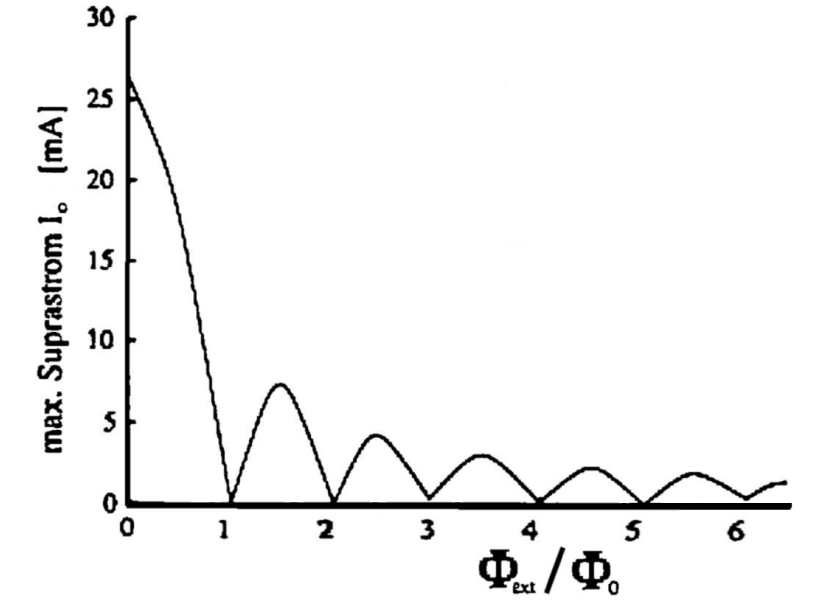
\includegraphics[scale=0.6]{Bilder/tstrom}
\caption{Maximaler Tunnelstrom durch den Josephson-Kontakt in Abhängigkeit des externen magnetischen Flusses. Quelle: [ver]}
\end{center}
\end{figure}
\section{Aufbau des Versuchs}
\begin{figure}[h]
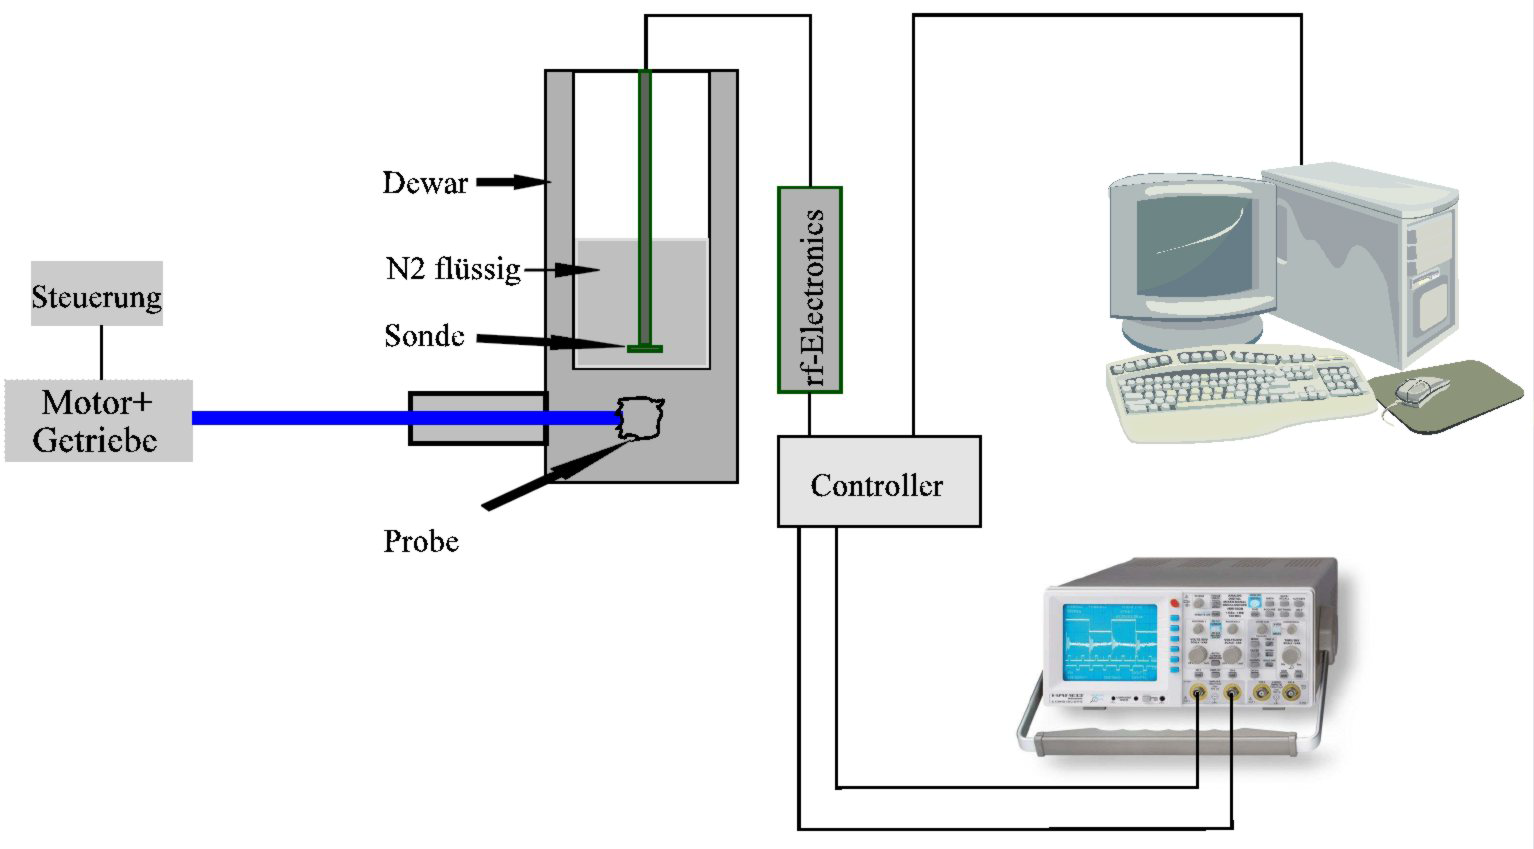
\includegraphics[scale=0.3]{Bilder/aufbau}
\caption{Aufbau. Quelle: [ver]}
\end{figure}
Im Versuch soll die Lebensdauer des durch Licht der Wellenlänge $253,7nm$ angeregten $^{3}P_{1}$-Zustandes von Quecksilber untersucht werden. Dazu benutzt man eine Quecksilberdampf- Niedrigdrucklampe (QL). Das so erzeugte Licht wird von der ersten Linse (L) kollimiert und von der zweiten fokussiert. Zwischen diesen Linsen ist ein Interferenzfilter (IF) angebracht, welche einen Durchlassbereich von $(255\pm5)nm$ FWHM  verwendet und somit die gewünschte Wellenlänge durchlässt. Besonders wichtig ist dabei, dass eine Wellenlänge von $184,5 nm$ herausgefiltert wird, da diese den sonst dominierenden Übergang von Quecksilber zwischen $^{1}P_{1}$ und $^{1}S_{0}$ anregen würde. Ein doppelbrechender Polarisationsfilter (PF) ermöglicht die Wahl der Polarisationsrichtung.\\
Das Licht trifft auf eine Quecksilberdampf-Resonanzzelle (QZ), welche aus einem Quarzkolben und einer Vertiefung im Boden besteht, in welcher sich das Quecksilber sammelt. Zur Kühlung der Zelle werden Peltierlemente (PE) verwendet. Aufgrund ihres elektrischen Störfeldes werden diese mithilfe wärmetransportierender 'Heat Pipes' (HP) möglichst weig weg von der Zelle positioniert. Ebenfalls außerhalb ist ein Photomultiplier (PM) angebracht, welcher über den Photoeffekt das Fluoreszenzlicht in ein elektrisches Signal umwandelt und durch einen Potentialgradienten und mehreren Elektroden das Signal verstärkt.\\
Zur Kompensation von Hintergrund-Magnetfeldern werden zwei Paare von Helmholtz-Spulen (HS) benutzt und ein drittes dient zum Durchfahren des magnetisches Feldes, welches für das Hanle-Signal sorgt.

\clearpage
\subsection{Winkelkorrelation von Vernichtungsphotonen}
Für die Messung der winkelabhängigen Koinzidenzen wurde für verschiedene Winkel mehrere Messungen mit einer Messdauer von jeweils 100s durchgeführt. Es wurde bei Winkeln von $-90^{\circ}$ bis $+90^{\circ}$ gemessen. Hierbei wurde der Plastikszintillator über einem Droharm in die jeweilige Position gebracht, wobei $0^{\circ}$ gerade einem Winkel von $180^{\circ}$ zwischen den beiden Szintillatoren entspricht.\\
An den Einkanaldiskriminatoren des NaJ-Szintillationszählers wurden die Energiefenster so eingestellt, dass möglichst nur Vernichtungsphotonen mit 511 keV registriert werden, d.h. es wurden nur Signale des Peak bei dieser Energie zum Zähler weiter geleitet.\\
Das Delay wurde mit Hilfe des Oszilloskops gewählt. Hierbei wurde die Speicherfunktion genutzt, somit konnte man eine Häufung der Signale feststellen und deren Verzögerung zum anderen festgehaltenen Signal auslesen und justieren.\\
Die Rate zu dein jeweiligen Winkeln berechnet sich wie folgt:
\[ n'(\phi)=\frac{\sum N_i(\phi)}{\sum t_i(\phi)} =: \frac{N_{ges}}{t_{ges}(\phi)} \]
wobei $N_i$ die Anzahl der Ereignisse der $i$-ten Messung und $t_i$ die Messzeit der $i$-ten Messung bei gleichem Winkel $\phi$ ist. Der Fehler der Gesamtrate $n'$ einer Winkeleinstellung $\phi$ lässt sich durch Fehlerfortpflanzung berechnen und erbigt sich durch:
\[ s_{n'}=\frac{1}{\sum t_i} \sqrt{\sum s_{N_i}^2~} = \frac{1}{t} \sqrt{\sum N_i~} = \frac{\sqrt{N}}{t}=\sqrt{\frac{n'}{t}} .\]
Der Fehler auf den Winkel wurde auf $s_{\phi}=0,5^{\circ}$ geschätzt. Die nicht eingekerbten Winkel wurden mit Hilfe einer selbst angefertigten Schablone realisiert. Durch fünf Messungen ohne Probe wurden die durch zufällige Koinzidenzen auftretenden Ereignisse und deren Zählraten bestimmt. Dieser Untergrund wurde von den gemessenen Werten abgezogen, wodurch sich der Fehler auf die vom Untergrund bereinigten Zählraten wie folgt berechnet:
\[ s_n=\sqrt{s_{n'}^2+s_u^2} \]
Auf die aufgetragenen Werte in Abb.\ref{fig:winkelkor} wurde eine Normalverteilung gefittet. 

\begin{figure}[h]
\begin{center}
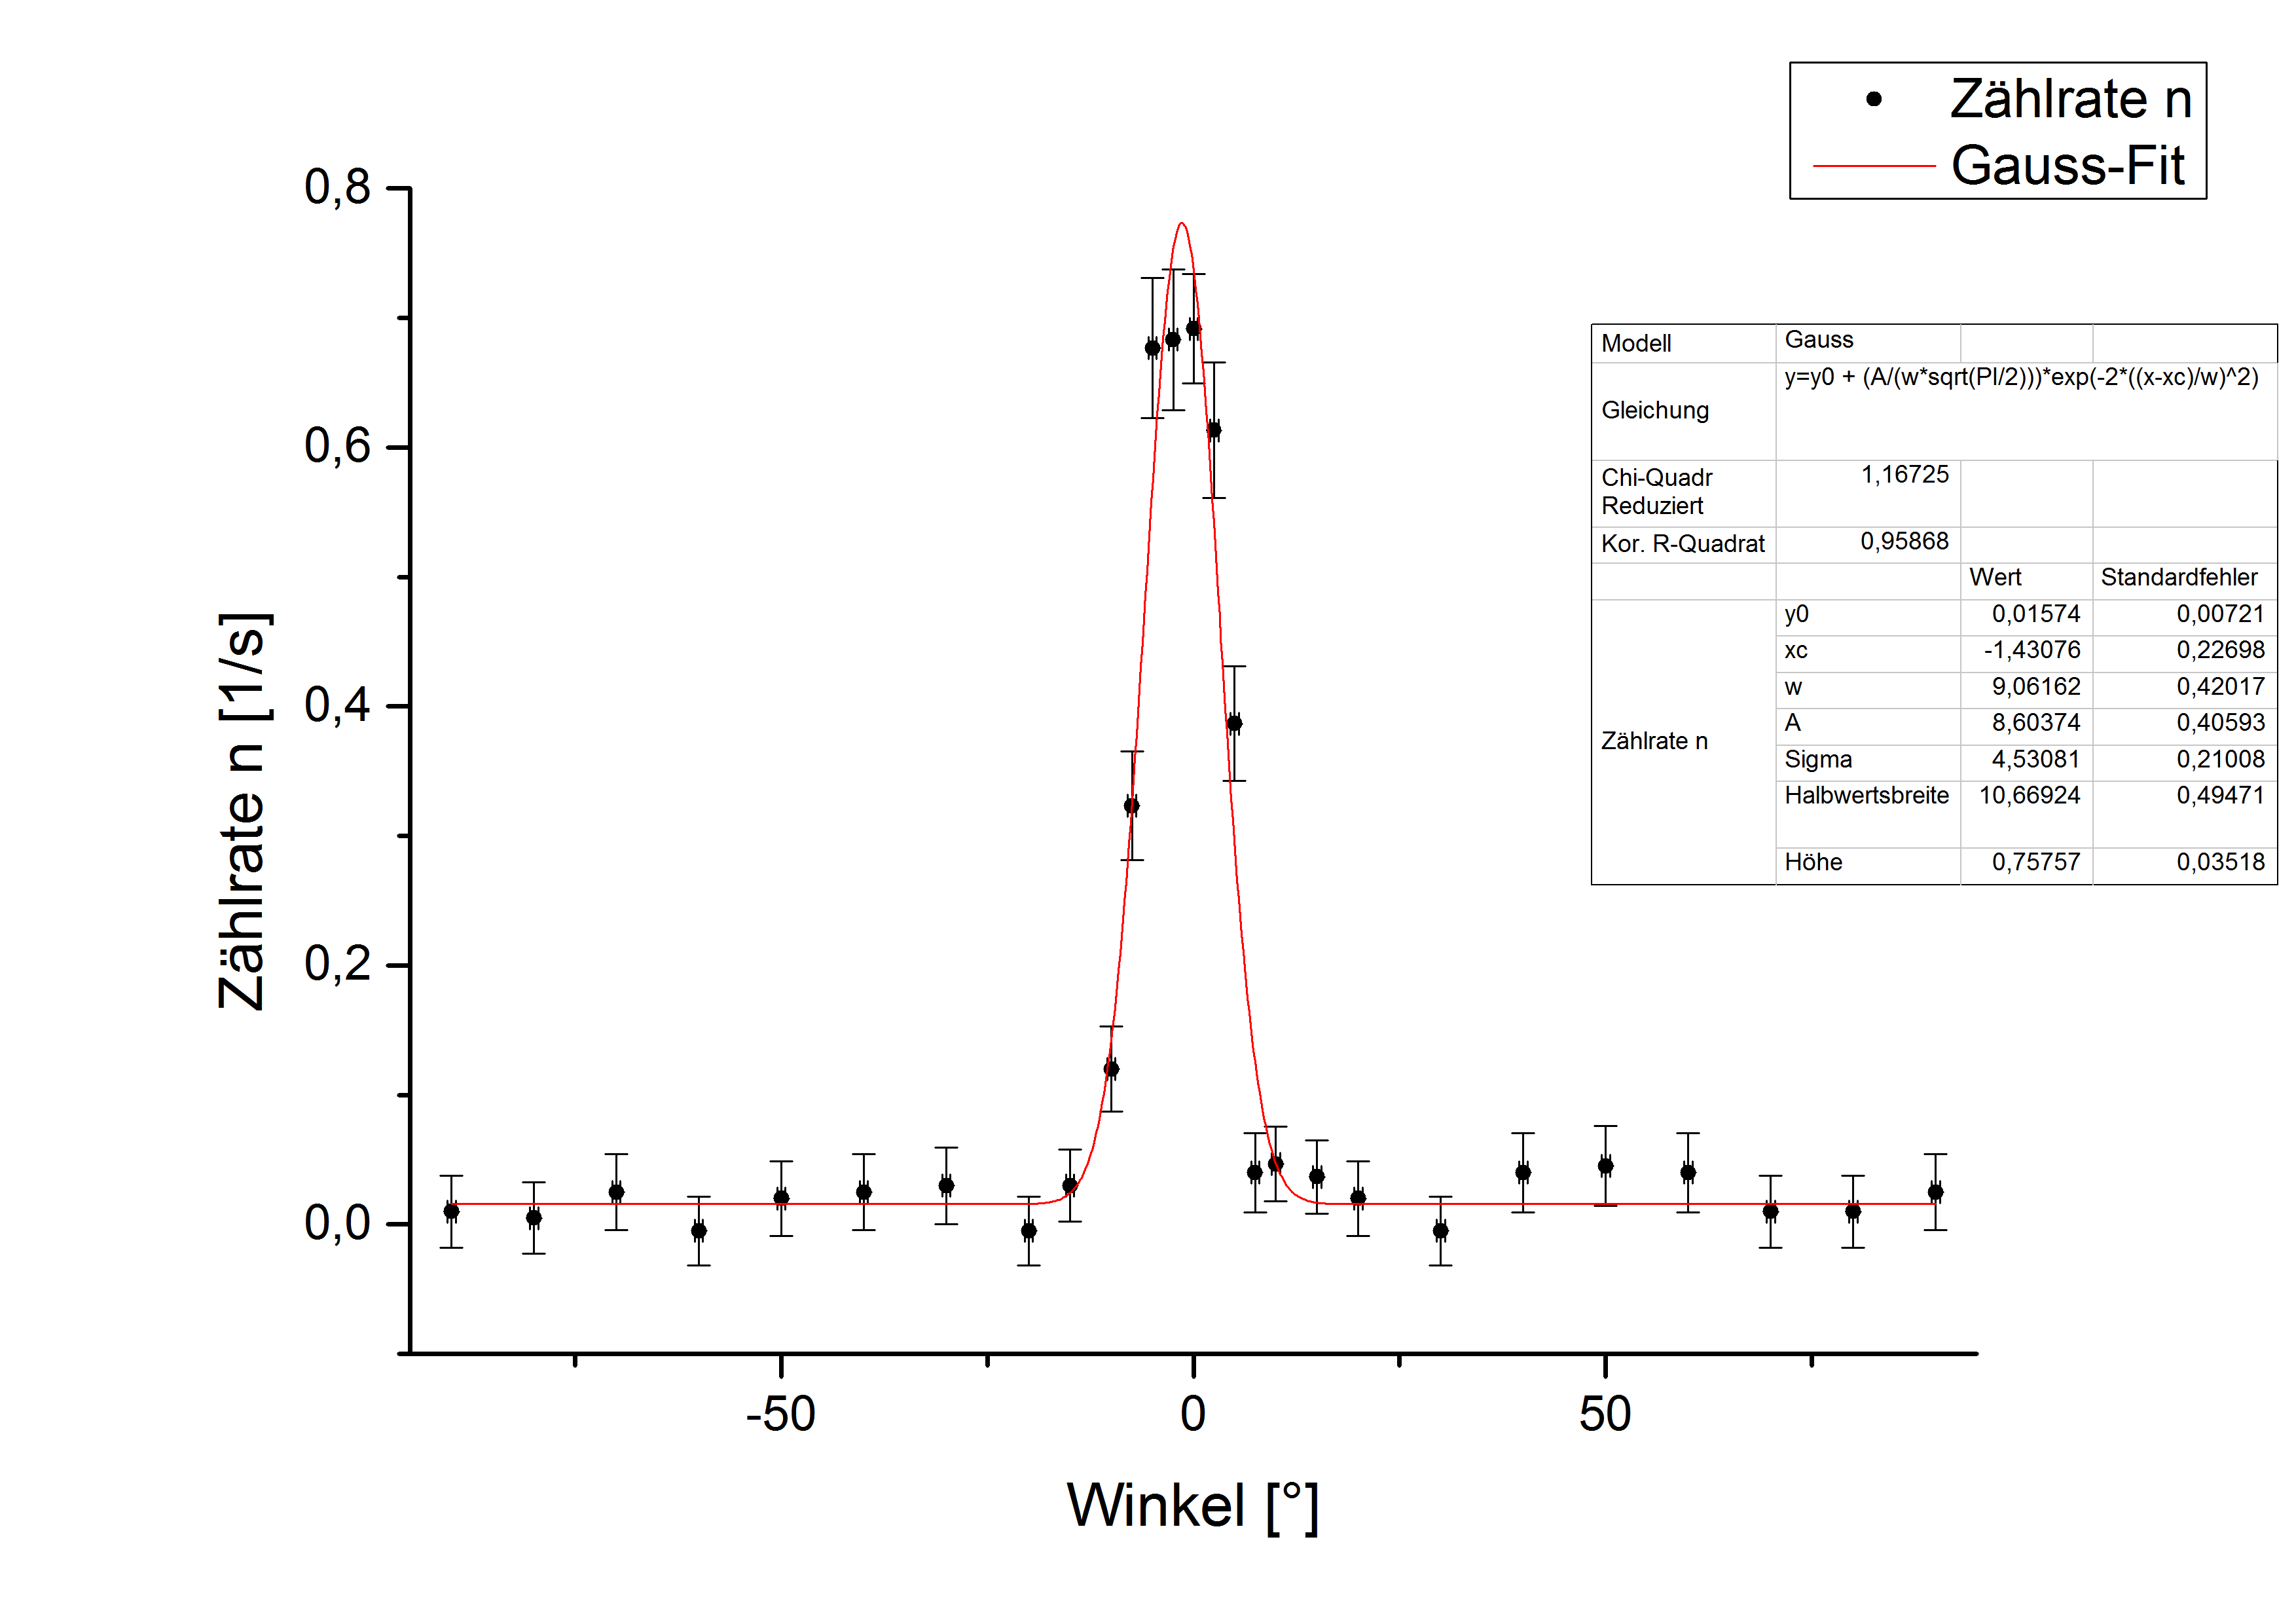
\includegraphics[scale=0.5]{winkelkor}
\caption{Winkelverteilung der Koinzidenzen.}
\label{fig:winkelkor}
\end{center}
\end{figure}

Der von uns gemessene Peak befindet sich bei einem Winkel von $\phi_0 = (-1,4\pm0,2)^{\circ}$ und somit im Rahmen der Messgenauigkeit nicht wie erwartet bei $0^{\circ}$. Diese Abweichung kann dadurch zu Stande kommen, dass die Drehachse nicht exakt zentriert war. Ein weiterer Grund könnte die kurze Messzeit sein, Zerfälle sind zeitlich statistische Ereignisse, für eine qualitativ bessere Aussage benötigt man eine längere Messdauer. In diesem Fall könnte unsere Abweichung eine zufällige Abweichung sein.
%Inhaltsverzeichnis
\end{document}
